\chapter{DTU Space coating facility}\label{chap:coating_facility}

The multilayer coating facility consists of a vacuum chamber placed in the laboratory known as the Multilab. It started out as a vapor deposition chamber for the SODART mission\cite{Christensen:1997kk,Schnopper:1994ip}. Capable of vaporising a gold wire with a W rod in the center of the chamber, it would deposit a layer of gold on any mirror facing the center. The chamber was later upgraded with magnetron cathodes, each with independent shutters.

The currently used cathodes are attached to powerful DC power supplies that can deposit films atom-by-atom instead of the larger gold particles that would come from vaporisation. The upgrade made it possible to coat multilayers with d-spacings thinner than 3 nm and eventually became the coating method used for the NuSTAR mission.

The entire lab was moved from Rockefeller Institute near Rigshospitalet in Copenhagen during the summer of 2012. It was up and running again around the summer of 2013 in the newly constructed building 328, the new home for DTU Space on DTU campus. In the new location, the lab is 50\% larger, has a double airlock (earlier just a single airlock), laminar airflow from ceiling mounted HEPA filters and various other improvements. The result is a considerably cleaner facility, which is important to avoid contaminants on optical substrates.

\begin{figure}[htbp]
  \centering
  \includegraphics[width=\linewidth]{figures/chamber/multilab1.png}
  \includegraphics[width=\linewidth]{figures/chamber/multilab2.png}
  \caption{\footnotesize Panoramic view of the Multilab coating facility at DTU Space. Top right can be seen the bell-shaped coating chamber.}
  \label{fig:multilab}
\end{figure}

The vacuum chamber is the dominant piece of the laboratory and most of the computers, electronics and cooling in the lab is in some way connected to the chamber. Apart from the chamber, the lab consists of a downflow module, two fume hoods, a profilometer, a large clean room oven and various tables and cupboards (see figure \ref{fig:multilab}). Next to the lab is the Multilab Auxiliary Room, which houses the cooling heat exchangers and pumps, the rotary vane roughing pump, DC power supplies, and a large part of the extra storage needed for the lab. Additionally, there is a room in the basement that houses a ceramic oven that has a built in vacuum chamber, the room also serves to store hundreds of spare pieces of NuSTAR optic glass.

\section{Coating chamber}
The coating facility at DTU Space is arranged with vertical sputtering cathodes pointing outwards in a circular vacuum chamber, see figure \ref{fig:chamber}. Substrates are mounted on vertical mounting plates that are placed on a rotating ring in the sputtering chamber and the substrates pass in front of each cathode at a speed determined by the desired layer thickness.

\begin{figure}[htbp]
  \centering  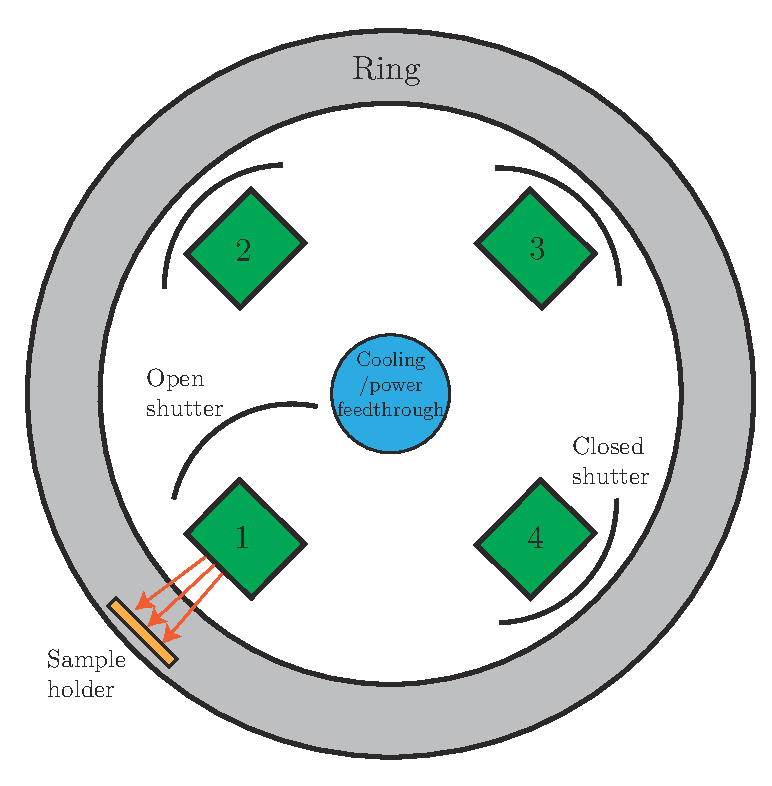
\includegraphics[width=0.5\linewidth]{figures/chamber/chamber.pdf}
  \caption{\footnotesize Diagram of the coating chamber at DTU Space, showing the principle of the rotating sample ring stage. Cathodes 1--4 (green) points outwards and can be covered with a shutter. Water cooling and power lines for the cathodes comes from the floor in the center of the chamber (blue) and connects to the top of each cathode with vacuum flex tubes. The sample (orange) is placed on a vertical plate that is mounted on the ring (grey). The ring rotates, so the samples move past the cathodes and gets coated with a film thickness related to the ring speed.}
  \label{fig:chamber}
\end{figure}

After chamber is closed, a roughing pump and a turbo molecular pumps evacuates the chamber to a pressure of $\leq2\cdot10^{-6}$ Torr before pure Ar gas is let into the chamber at a constant flow rate to ensure the fraction of other gases to be $<$0.1\%. The desired total pressure with Ar gas is $2.8\cdot10^{-3}$ Torr, which is as low as possible while maintaining plasma stability.

The chamber fits four cathodes at a time and the Multilab has six in total, so two can be serviced while the other four are in use. For most coatings, only two or three cathodes at a time are necessary for the same number of materials.

In the earlier software solution, all cathodes were switched on at the same time during deposition of a bilayer. That necessitated two cathodes running with the low-Z material while one cathode ran with the high-Z material in order to achieve the correct $\Gamma$ value and to have each cathode running in a possible power regime. A typical Pt/C  multilayer for NuSTAR required $\Gamma = 0.6$, which meant that 60\% of a material in a bilayer had to be carbon. Platinum and carbon has vastly different coating rates, so one cathode with Pt running at 150 W required two cathodes of C running at 900 W in order to achieve $\Gamma = 0.6$. With the new software only one cathode with each kind of material is necessary, but at the expense of a longer coating time.

\subsection{Magnetron cathodes}
The cathodes are the most important part of the chamber. They are 20 inches long and 1/2 inch wide planar magnetron cathodes made by Angstrom Sciences Inc. A diagram of the cathode can be seen in figure \ref{fig:cathodeintersection}. A copper (Cu) block acts as the cathode with a stainless steel shield around it, separated by teflon spacers. Inside the Cu block, three permanent magnets with alternating field directions supplies a magnetic field in front of the cathode. Water cooling and power lines are connected from the cathode through a flexible vacuum tube to water cooling and power supplies outside the chamber. The anode shield is grounded along with the rest of the chamber.

\begin{figure}[htbp]
  \centering  \includegraphics[width=0.5\linewidth]{figures/chamber/cathodeintersection.pdf}
  \caption{\footnotesize Cross-sectional diagram of a magnetron cathode used in the Multilab at DTU Space. }
  \label{fig:cathodeintersection}
\end{figure}

Materials for sputtering, called targets, are fastened to the Cu block using a stainless steel clamp. It is important for the target to have a uniform contact with the cathode, so the Cu block should be cleaned before fastening using cleanroom wipes and ethanol. For tougher blemishes, a micro-fine sanding sponge can be used to clean the surface followed by ethanol and cleanroom wipes.

Applying a voltage of -400 V to the cathode creates an electric field in front of the target. The Ar gas present in the chamber will be ionised in front of the cathode by the electric field, stripping an electron from the Ar atoms resulting in a plasma. The positive Ar$^+$ ions are accelerated towards the target, whereby the collision with the target create a sputtering of target atoms in a cone directed normal to the target surface, see figure \ref{fig:sputtering}. A substrate placed opposite the cathode will be coated with the sputtered atoms at a rate proportional to the electric current applied to the cathode.

\begin{figure}[htbp]
  \centering  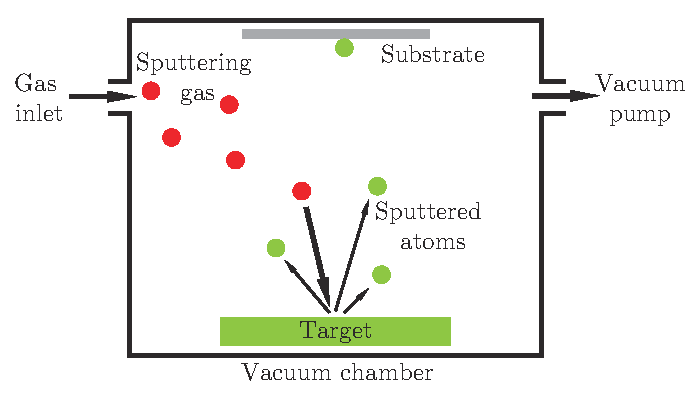
\includegraphics[width=0.6\linewidth]{figures/chamber/sputtering.pdf}
  \caption{\footnotesize Principle of sputtering. Sputter gas led into an evacuated chamber is forced to the surface of a target with a force that rips atoms from the material. The freed target atoms move away from the target and some hit a substrate opposite the target. }
  \label{fig:sputtering}
\end{figure}

Electrons stripped from Ar atoms are captured by the magnetic field lines from the permanent magnets in the Cu block. The electrons are moved back and forth across the target and occasionally hits neutral Ar atoms, which also become ionised and thereby sustain the plasma. The movement of electrons are from the center of the target to the outer edge, and as more Ar atoms are ionised in between those two points, the main erosion of the target during coating takes place in a so-called \emph{race track} around the target.
%
% !!!!!Something about the physics of sputtering!!!!!
%
% !!!!Thornton zone model?????!!!!!!

\section{Multilab control software}\label{sec:ml_software}
In the years before moving the DTU Space multilab to DTU campus, it became apparent that a completely new software solution was needed for the coating facility. The software controls all stepper motors (cathode shutters and sample ring), gas flow controllers,  cathode power supplies as well as pressure gauge communication.

The original software was made in Visual Basic 6, which Microsoft stopped supporting in 2008. Features that were not build into the software from the start was bolted on at a later stage, resulting in some files with thousands of lines of uncommented code. VB6 also has the drawback that it is single threaded, so only one command can be executed at a time which means that none of the instruments could be read for the log file if for instance the sample ring was moving. So checking whether there was a plasma dropout on a cathode was not possible while coating a layer, something that can take 30+ minutes.

Everything in the original software solution was controlled in a graphical user interface which made it easy to use, but would only allow for preprogrammed coating types to be made. When it came to make coating investigations for the ATHENA mission, the linearly graded coatings with top and bilayer required being in front of the computer during the process. For every layer, it was necessary to manually type in a new sample ring speed and start the movement. The coatings took on average 2-3 hours, so it became clear that a new solution was necessary.

\subsection{Considerations on the new software solution}
Considering the observations from above, a list of requirements for new software was made:

\begin{description}
  \item[Software should run on Linux] To remote control the coating facility in the old software solution, it was necessary to run a remote desktop to control the graphical user interface. The remote desktop requires a relatively large amount of internet bandwidth, something that is not always available. The new software should be controllable over a remote SSH connection using a Bash shell or similar.
  \item[Software should log continuously] Output from cathode power supplies, pressure gauges and flow meters should be read every 5 seconds during a coating. Between coatings, the pressure gauges should be read every 5 seconds and written to a web server. That allows for checking chamber status on a smart phone or computer connected to the internet.
  \item[A coating run should be described in a script] Instead of predefined coating types, the scripts make it possible to produce completely custom multilayer coatings.
  \item[Software should preferably be open source] Open source software is often well documented and flexible. An open source programming language with plenty of extra packages could be Python.
\end{description}

The first attempts at creating new software was directed at Python, since that is just about the most well-documented programming language on the internet, and also where I have the most experience.

It became clear after a while that the real problem was satisfying the second requirement in the list above. All instruments controlled by computer in the multilab are communicated with using serial connections, which will block a line until a command is received by an instrument and a response is returned. In some instruments the response time is up to a second and for the stepper motors, a response is not returned until movement is complete. That is the reason why the old software was unable to read any outputs during the movement of the sample ring.

Python is a single threaded scripting language, so all commands are executed sequentially. There are however software packages for Python that can spawn subprocesses from a queue and read the output of those into another queue. A specific package for multithreading serial communication is Twisted for Python, but after moderately successful attempts it was clear that the solution would be too difficult. The software should be flexible and making a multithreaded python solution with queue systems was both too much work and a bit like reinventing the wheel.

The choice in the end fell on SPEC, a software package for X-ray diffraction setups. SPEC is not open source, but requires a license. SPEC is widely used in synchrotron beamlines across the world, and also in the X-ray lab at DTU Space. It is an extremely flexible piece of software, specifically designed to talk to a wide range of instruments at X-ray beamlines. Many types of hardware can be controlled directly from SPEC without the need for drivers, since a direct hardware level communication protocol is build into the software. Commands are typed in on a command line, but can also written into text files (scripts) and the commands can then be executed sequentially by SPEC.

\subsection{Software architecture of new Multilab control program}
SPEC is, like Python, single threaded. There are however build-in procedures for communicating through the serial protocol and a range of other protocols. SPEC also has the ability to run as a server so commands can be issued to the software using sockets on the system level. By running three separate instances of SPEC at the same time, it became possible to constantly communicate with instruments, write to a logfile, and control the chamber from a main program. The software is set up like the following:

\begin{description}
  \item[SPEC (main program)] The main program, where user-level commands can be typed in. Coating macros are executed from this program. The program has direct control with stepper motors using text-based serial communication\footnote{To use SPEC most efficiently, a direct hardware-level communication should be initiated between SPEC and motor controller. However, the motor controller would have to be supported on the hardware-level by SPEC, which is not the case for the current hardware in the Multilab. If a new motor controller is procured, it should be on the list of hardware supported by SPEC. (\emph{http://www.certif.com/hdwdevices.php?family=motor})}.
  \item[ControlServer] The control program. It has direct access to cathode power supplies, gas flow controllers and pressure gauges. SPEC and LogClient will get status and control the instruments through ControlServer by socket commands.
  \item[LogClient] The logging program. It gets data from the ControlServer every five seconds and writes the data to a file. If a coating is starting, it will make a new folder in the \verb'~/logs' directory named by time and date. In that directory it will make a log file (\verb'logfile.txt') for the coating and also a log of the commands typed in by a coating macro (\verb'coatinglog.txt').
\end{description}

These three programs run continuously side-by-side, and will make sure that there are no interruptions in the logging during a coating run. Each command to control any part of the instruments are described in the \verb'site.mac' macro files of each program and auxiliary macro files for e.g. power supplies and pressure gauges. All commands are divided into system-level and user-level commands. System-level commands are called like this:

\begin{verbcode}
  SPEC> output = getpoweroutput(#)
\end{verbcode}

This command will get the output of cathode \verb'#' and put the result in the variable \verb'output'. The system-level commands \emph{can} be used by the user, but \emph{should not}. Instead they are used inside user-level command macros, so a user-level command looks like this:

\begin{verbcode}
  SPEC> getpoweroutput 1
  Current power output of cathode 1: 450 W
\end{verbcode}

This makes it easier to type commands into SPEC, as commands can be autocompleted by using the tabulator key. If a command needs one or several parameters following it and not enough/too many are given, it will respond with an error and a description of the parameters needed.

Log files produced continuously by the LogClient program are fetched by a web server at DTU Space that will make a plot of pressure and cathode power output every 30 seconds. A plot from Sept. 14th 2014 can be seen in figure \ref{fig:chamber_pressure}. The logfile holds up to 50,000 lines of data, which corresponds to $\sim$3 days of data collected every five seconds. In the plot can be seen both the curve corresponding to the cold cathode pressure gauge (red line) and the baratron pressure gauge (green line). The cold cathode works well at both low and high pressure, but some of the functional parts can be coated over during a coating, so a valve closes off to that gauge during coating. The baratron only works between $10^{-1}$ Torr and $2\cdot10^{-4}$ Torr, but is more precise and also works during a coating.

\begin{figure}[htbp]
  \centering
    \includegraphics[width=0.8\linewidth]{figures/chamber/pressure.png}
  \caption{\footnotesize Plot representing the output from the continuous logging of chamber pressure. Red line is the pressure measured by a combined cold-cathode/penning gauge, that works well under both atmospheric pressure and low pressure. It will not function well during a coating. Green line is the MKS Baratron pressure gauge, that is precise in the $2\cdot10^{-4}$ -- $5\cdot10^{-2}$ Torr range.}
  \label{fig:chamber_pressure}
\end{figure}

The web server that continuously fetches the log file from the coating computer also gets information from the X-ray measurement computer in the basement. Information about measurement status and progress is posted to the same web site. This makes it possible to get the status about all the labs by a quick glance to the web site. The script running on the web server also has the option to send out a mail to pre-defined recipients if the pressure in the chamber is low enough to start a coating. This proved handy during the NuSTAR coatings, where coatings had to be started in the middle of the night. The web site and script running on the web server were produced during the NuSTAR coating campaign to make the production process easier.

The cathode shutters and ring are all controlled by the same motor controller, and is communicated to over the same serial cable. That is however opaque to the user. In order to open or close a specific shutter, the command \verb'osh #' or \verb'csh #' should be given for opening and closing shutter \verb'#', respectively. Alternatively, all shutters can be opened or closed using \verb'openallshutters' and \verb'closeallshutters'. The ring can be controlled using the commands \verb'mra speed angle' or \verb'mr speed steps', the first of which moves the ring at the speed given in steps/sec. at an angle given in degrees. The second does the same thing, except for changing the angle for steps. The motor controller has 668,000 steps in a complete rotation of the ring in the chamber and the speed of the ring should be between 0 and 15,000 steps/sec, otherwise the movement precision decreases. In a coating macro, the command \verb'mra speed angle' is used extensively as the main method to move the samples past the cathodes.% In chapter \ref{chap:multilab_details}, an extensive list of commands made for the control software can be found.

\subsubsection{Interfacing with cathode power supplies}
The power supplies used to run the cathodes in the multilab consist of two Advanced Energy Pinnacle 5/5 DC power supplies and one Advanced Energy Pinnacle Plus+ 5/5 pulsed-DC power supply. Each power supply has two channels, so can run two cathodes at same time. In order to communicate with power supplies, a special protocol running over serial has to be used. All other instruments in the multilab are communicated with by ControlServer and SPEC using basic text commands send over a serial connection.

The protocol is made for connecting all power supplies to the same serial connection, but in the multilab they are connected separately. The protocol requires each command to be packaged in a binary packet that includes power supply hardware address, length of packet, command, data and finally an XOR of the entire packet so the receiver can verify that the whole packet is there. The design of the packet can be seen in figure \ref{fig:ae_packet}. In the header, which is 8 bits long, the first 5 are the address of the power supply (set with a DIP switch on the back) and the remaining 3 bits describe the length of the packet. If the length in the header is set to 7 (111 in binary), the 'optional' byte is used to describe the actual length of the packet. The 'command' byte is a number between 0 and 255 (0 and FFh) in hexadecimal numbers. The 'checksum' byte is an XOR of the entire packet up until the 'chekcksum' byte. When the receiver gets a packet, it will do an XOR of the entire packet including the 'checksum' byte and if the result is 0, the packet is approved and processed.

\begin{figure}[!h]
  \center
  \includegraphics[width=0.9\linewidth]{figures/chamber/ae_packet.pdf}
\caption{\footnotesize Schematic of the principle of transmission data packets in the Advanced Energy communication protocol. Each number on the white line corresponds to one bit in the data packet, eight bits equals one byte. From \cite{Anonymous:zazNQqcS}}\label{fig:ae_packet}
\end{figure}

This packet architecture is used to communicate back and forth between the ControlServer program and the power supplies. If a packet is approved, an ACK is send back in the form of the hex code 06h. The commands for the power supplies can either be to retrieve current status of some parameter, to set a parameter on the power supply, or to execute a command on the power supply. The entire communication protocol is transparent to the user and all user-level control of the power supplies can be achieved by user-level commands only.

\subsubsection{Coating macro}
To produce a coating in the multilab chamber, a coating macro can be typed up and started in the main SPEC program as soon as the pressure is low enough ($\leq2\cdot10^{-6}$ Torr). An example of a simple coating macro, \verb'coat_singlelayer', can be seen here:

\begin{verbcode}
  def coat_singlelayer '
        if ($# != 1) {
                eprint "Start coating of singlelayer.\n"
                eprint "Usage: coat_singlelayer v(cath3)"
                exit
        }
        coating_start_log
        closevalve
        setflow 1 88
        openflow 1
        openmainflow
        print("Waiting for Ar flow to settle.\n")
        print("(60 seconds).\n")
        sleep(60)
        setpower 3 450
        print("Starting coating.\n")
        mra 90 10000
        sleep(2)
        pson 3
        sleep(5)
        osh 1
        print("Coating material 1, all plates.\n")
        mra -360 $1
        sleep(2)
        csh 1
        sleep(1)
        psoff 3
        mra -90 10000
        sleep(2)
        print("Coating over. Closing flow valve.\n")
        closemainflow
        closeflow 1
        openvalve
        coating_stop_log
\end{verbcode}

Each step in the macro is described here:

\begin{description}
  \item[Error check] The macro starts out with an \verb|if| statement to make sure that there is one parameter after the user has called the macro.
  \item[coating\_start\_log] Sets the variable \verb|coating_starting=1| in the LogClient program and lets it know that it is time to start a log for a new coating.
  \item[closevalve] Closes valve to the cold cathode pressure gauge.
  \item[setflow 1 88] Sets flow output on flow controller 1 to 88 SCCM.
  \item[openflow 1] Opens flow controller 1.
  \item[openmainflow] Opens flow controllers to chamber.
  \item[Text output to user] Feedback should be given to user throughout the coating.
  \item[sleep(60)] Macro will wait for 60 seconds to let the pressure settle at $\sim$2.8 mTorr.
  \item[setpower 3 450] Power output is set to 450 W on power supply output 3, the first output on the second power supply.
  \item[mra 90 10000] Ring is moved 90\degr\ at a speed of 10,000 steps/sec. so the first sample is right before cathode 1.
  \item[pson 3] Power supply 3 is turned on.
  \item[osh 1] Shutter 1 to cathode 1 is opened.
  \item[mra -360 \$1] Ring is moved 360\degr\ at the speed given by the parameter which is set by the user when calling the macro.
  \item[csh 1] Shutter 1 is closed after ring is done moving.
  \item[psoff 3] Power supply 3 is turned off.
  \item[mra -90 10000] Ring is moved back to start position.
  \item[closemainflow] Main flow to flow controllers is turned off.
  \item[closeflow 1] Flow controller 1 flow is turned off.
  \item[openvalve] Valve to cold cathode pressure gauge is opened.
  \item[coating\_stop\_log] Sets the parameter \verb|coating_starting=0| in the LogClient program, which stops logging for that coating.
\end{description}

The macro will coat all samples in the ring with one layer of the material on cathode 1 at the speed given by the parameter after the macro call. Macros in SPEC are given in a C-type language and many types of loops and statements are implemented. The comprehensive manual for SPEC gives a good overview.

If the user wants to make more complicated multilayers, adjusting the macro example above into a graded-d type coating can of course seem daunting. For that reason, subfunctions are implemented that will coat e.g. 90\degr\ of the ring with cathode 3. The principle of the subfunction is as follows:

\begin{enumerate}
  \item From the start position of the ring where sample 1 is placed, the ring will move sample 1 between cathode 2 and 3.
  \item Turn on cathode 3 and open shutter.
  \item Move ring 90\degr\ given by input parameter.
  \item Close shutter 3 and turn off cathode.
  \item Move ring back to start position.
\end{enumerate}

The sample can then be coated by another cathode afterwards. If a larger batch requires coating at the same time, there are similar subfunctions for moving 180\degr\ and 360\degr.

The software also makes it possible to coat four different samples with four different coatings in the same coating run. By placing the samples at four different corners of the ring, each sample can have a coating applied separately. Flexible macros for that purpose are not yet implemented, but a template that can be changed into a specific purpose is the macro
\begin{verbcode}
  SPEC> coat_n_bilayers_4plates
\end{verbcode}
along with subfunction e.g.
\begin{verbcode}
  SPEC> abilayer_4_plates_c2c4($2,$3,$4,$5,$6,$7,$8,$9)
\end{verbcode}
that will coat four different constant-d coatings using cathode 2 and 4. It is possible to change any parameter for the power supplies or flow meters between each sample, so testing out a parameter space becomes significantly faster with this system.

For linearly graded-d coatings, an example is given below that shows the flexibility of the SPEC macro language.

\begin{verbcode}
  for (j=0;j<nlayers;j++){
    printf("\nStarting layer %g.\n",j+1)
    dlayer = dmin+(j)*(dmax-dmin)/(nlayers-1)
    dlayer1 = dlayer*gamma
    dlayer2 = dlayer*(1-gamma)
    speed1 = int(1/((dlayer1-sicorr)/sifact))
    speed2 = int(1/((dlayer2-wcorr)/wfact))
    coat_cath2_180 speed2
    coat_cath4_180 speed1
    }
\end{verbcode}

By defining \verb|nlayers| as the number of layers, \verb|dmin|, \verb|dmax| and \verb|gamma| of the coating along with calibration factors, the macro will for every layer calculate the speed for both materials and coat the correct thickness. Calibration factors are calculated as seen in section \ref{sec:coating_calib} where $a$ for W is \verb|wfact| and $b$ is \verb|wcorr|. The same principle can be used in other types of graded-d coatings, e.g. power-law gradings with $a$, $b$ and $c$ defined in $d_i = a/(b+i)^c$, where $d_i$ is the d-spacing of the i'th layer.

\section{X-ray lab source at DTU Space}
Measurements at DTU Space were done with a reflectivity setup consisting of a rotating Cu-anode providing X-ray photons for two beams. One beam is used for reflectivity measurements and the other can be set up for measuring curvature in glass substrates.

After the source, along the z-axis, is placed two slits, a monochromator, an attenuator, on more slit, the sample holder and finally the detector, see figure \ref{fig:xraysetup}. The first two slits ensures that only a narrow beam hits the monochromator, which then reflects only photons around the Cu K$_{\alpha_1}$ emission line (8.047 keV) by reflecting the beam on two Ge crystals at an angle where Bragg reflection only allow photons of that energy. The beam continues through the next two slits, thereby minimizing divergence and also filters out a large part of unwanted reflections from the monochromator to ensure a narrow bandwidth. The attenuator ensures that the beam intensity is not too large, thereby saturating the detector.

\begin{figure}[!h]
  \center
  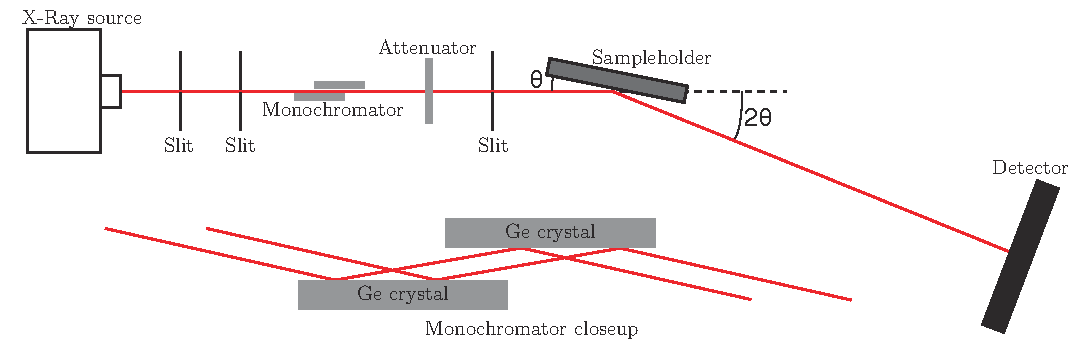
\includegraphics[width=0.8\linewidth]{figures/chamber/xraysetup.pdf}
\caption{\footnotesize Diagram of the X-ray setup at DTU Space. X-ray photons from the source goes through two slits, a monochromator, an attenuator and one more slit before hitting the sample. The reflected photons from the sample travel to the detector which is rotated at a $2\theta$ angle. Below: The monochromator that consists of two Ge crystal that reflect only a given wavelength on the (111) surface using the Bragg principle.}\label{fig:xraysetup}
\end{figure}

The sample holder consists of a slab of flat perforated ceramic material, a vacuum chuck, mounted vertically. It is connected to a pump, which allows flat substrates, like pieces of Si-wafer, to stick very firmly to the stone slab. This method of sample mounting makes it possible to change samples very fast and easy between measurements. The sample holder is centered and mounted on a rotating stage, $\theta$, and can also move in and out of the beam along the x-axis.\\
After the sample holder, 995 mm further along the z-axis is a 10 cm wide 2D methane-gas detector mounted on a rotating stage, $2\theta$. It is centered on the same axis as $\theta$, allowing the detector to move 90\degr around the sample while maintaining a focus on the same spot. The detector has 2000 channels along the x-axis of the beam; 100 channels are used during a measurement, giving a horizontal detector aperture of 2 cm.

\section{Coating calibration}\label{sec:coating_calib}
To deposit a coating with the correct film layer thicknesses on a substrate, a calibration of the material combination is required. Four samples of 10 bilayer films are coated using the two materials. Each sample is placed on a separate mounting plate and each coated with a different thickness of both light and heavy materials. The samples are then measured using XRR and compared to an IMD\cite{Windt:1998tb} model fit to get bilayer thickness (d-spacing) and light/heavy material fraction ($\Gamma$) as seen in figure \ref{fig:irb4c-fit}.

\begin{figure}[!h]
  \center
  \includegraphics[height=7cm]{figures/chamber/si5811-fit.pdf}
\caption{\footnotesize XRR measurement of a 10 bilayer Ir/B$_4$C coating to calibrate for SPO coating. The measurement is fitted with an IMD model to determine d-spacing $\Gamma$.}\label{fig:irb4c-fit}
\end{figure}

The result for each sample is used to get the specific thickness of a material when coating with a given speed. Each result from the IMD model fitting is put into a table like the following:

%\begin{table}[!h]
\begin{center}
\begin{tabular}{c|c|c|c|c}
Sample & speed (Ir) & speed (B$_4$C) & d-Ir [nm] & d-B$_4$C [nm] \\
\hline
si5809 & 2623 & 473 & 2.42 & 2.54 \\
si5810 & 1445 & 338 & 3.21 & 3.88 \\
si5811 & 1011 & 236 & 4.33 & 5.81 \\
si5812 &  674 & 158 & 6.40 & 8.85 \\
si5813 & 281 & 225 & 14.55 & 7.49
\end{tabular}
\end{center}
%\caption{\footnotesize Calibration samples coated with 10 bilayer Ir/B$_4$C multilayers of different thickness. Each sample is measured using XRR and fitted to an IMD model. \label{tab:AFMsamples}}
%\end{table}

The d-spacings for a given material are plotted as a function of the inverse speed of the sample ring (v$^{-1}$) and fitted with a linear regression as seen in figure \ref{fig:calib-fit}. The $a$ and $b$ values of the linear regression are used directly to determine the speed of the sample ring, $v_{\mathrm{B}_4\mathrm{C}}$, to coat e.g. B$_4$C with a thickness of $d_{\mathrm{B}_4\mathrm{C}}$ like so:

\begin{eqnarray}
	v_{\mathrm{B}_4\mathrm{C}} = \frac{a}{d_{\mathrm{B}_4\mathrm{C}}-b}.
\end{eqnarray}

\begin{figure}[!h]
	\center
\includegraphics[width=0.8\linewidth]{figures/chamber/calibration_plot-ir-b4c.pdf}
\includegraphics[width=0.8\linewidth]{figures/chamber/calibration_plot-w-si.pdf}
\caption{\footnotesize Linear regression fits of calibration samples for Ir/B$_4$C (top) W/Si (bottom). Each datapoint is the XRR measured thickness of one material layer in a sample.}\label{fig:calib-fit}
\end{figure}
